% **** Szablon pracy magisterskiej, licencjackiej lub inżynierskiej ****

\documentclass[polish,12pt,twoside,a4paper]{report}

% *************** Definicje stylu dokumentu ***************

% *********************************************************************************
% W pliku tym zdefiniowany jest wygl¹d dokumentu.
% Zmiany tutaj nie s¹ konieczne o ile nie zamierzasz zmieniaæ wygl¹du dokumentu.
% *********************************************************************************

% *************** Za³adowanie pakietów ***************
\usepackage[a4paper,twoside,left=2.0cm,right=1.5cm,top=1.5cm,bottom=1.5cm]{geometry}
\usepackage[T1]{fontenc}
%\usepackage[cp1250]{inputenc}
\usepackage[utf8]{inputenc}
\usepackage[polish]{babel}
\usepackage{amsmath}
\usepackage{amsfonts}
\usepackage{graphicx}
\usepackage{graphics}
\usepackage{times}
\usepackage{url}
\usepackage{indentfirst}%wciecia a nowych akapitach
\usepackage{float}
\selectlanguage{polish}

%szerokoœœ wciêæ
\setlength{\parindent}{1.25cm}

%numeracja stron
\usepackage{fancyhdr}
\pagestyle{fancy}
\fancyhf{} % usun biezace ustawienia pagin
\fancyhead[LE,RO]{ }
\fancyhead[LO]{ }
\fancyhead[RE]{ }
\fancyfoot[LE,RO]{\small\thepage}
\fancyfoot[LO]{ }
\fancyfoot[RE]{ }
\renewcommand{\headrulewidth}{0.0pt}
\renewcommand{\footrulewidth}{0.0pt}
\addtolength{\headheight}{0.0pt} % pionowy odstep na kreske
\fancypagestyle{plain}{%
\fancyhead{} % usun p. górne na stronach pozbawionych
% numeracji (plain)
\renewcommand{\headrulewidth}{0.0pt} % pozioma kreska
}

% *************** Definicje niektórych kolorów ***************
\usepackage{color}

\definecolor{greenyellow}   {cmyk}{0.15, 0   , 0.69, 0   }
\definecolor{yellow}        {cmyk}{0   , 0   , 1   , 0   }
\definecolor{goldenrod}     {cmyk}{0   , 0.10, 0.84, 0   }
\definecolor{dandelion}     {cmyk}{0   , 0.29, 0.84, 0   }
\definecolor{apricot}       {cmyk}{0   , 0.32, 0.52, 0   }
\definecolor{peach}         {cmyk}{0   , 0.50, 0.70, 0   }
\definecolor{melon}         {cmyk}{0   , 0.46, 0.50, 0   }
\definecolor{yelloworange}  {cmyk}{0   , 0.42, 1   , 0   }
\definecolor{orange}        {cmyk}{0   , 0.61, 0.87, 0   }
\definecolor{burntorange}   {cmyk}{0   , 0.51, 1   , 0   }
\definecolor{bittersweet}   {cmyk}{0   , 0.75, 1   , 0.24}
\definecolor{redorange}     {cmyk}{0   , 0.77, 0.87, 0   }
\definecolor{mahogany}      {cmyk}{0   , 0.85, 0.87, 0.35}
\definecolor{maroon}        {cmyk}{0   , 0.87, 0.68, 0.32}
\definecolor{brickred}      {cmyk}{0   , 0.89, 0.94, 0.28}
\definecolor{red}           {cmyk}{0   , 1   , 1   , 0   }
\definecolor{orangered}     {cmyk}{0   , 1   , 0.50, 0   }
\definecolor{rubinered}     {cmyk}{0   , 1   , 0.13, 0   }
\definecolor{wildstrawberry}{cmyk}{0   , 0.96, 0.39, 0   }
\definecolor{salmon}        {cmyk}{0   , 0.53, 0.38, 0   }
\definecolor{carnationpink} {cmyk}{0   , 0.63, 0   , 0   }
\definecolor{magenta}       {cmyk}{0   , 1   , 0   , 0   }
\definecolor{violetred}     {cmyk}{0   , 0.81, 0   , 0   }
\definecolor{rhodamine}     {cmyk}{0   , 0.82, 0   , 0   }
\definecolor{mulberry}      {cmyk}{0.34, 0.90, 0   , 0.02}
\definecolor{redviolet}     {cmyk}{0.07, 0.90, 0   , 0.34}
\definecolor{fuchsia}       {cmyk}{0.47, 0.91, 0   , 0.08}
\definecolor{lavender}      {cmyk}{0   , 0.48, 0   , 0   }
\definecolor{thistle}       {cmyk}{0.12, 0.59, 0   , 0   }
\definecolor{orchid}        {cmyk}{0.32, 0.64, 0   , 0   }
\definecolor{darkorchid}    {cmyk}{0.40, 0.80, 0.20, 0   }
\definecolor{purple}        {cmyk}{0.45, 0.86, 0   , 0   }
\definecolor{plum}          {cmyk}{0.50, 1   , 0   , 0   }
\definecolor{violet}        {cmyk}{0.79, 0.88, 0   , 0   }
\definecolor{royalpurple}   {cmyk}{0.75, 0.90, 0   , 0   }
\definecolor{blueviolet}    {cmyk}{0.86, 0.91, 0   , 0.04}
\definecolor{periwinkle}    {cmyk}{0.57, 0.55, 0   , 0   }
\definecolor{cadetblue}     {cmyk}{0.62, 0.57, 0.23, 0   }
\definecolor{cornflowerblue}{cmyk}{0.65, 0.13, 0   , 0   }
\definecolor{midnightblue}  {cmyk}{0.98, 0.13, 0   , 0.43}
\definecolor{navyblue}      {cmyk}{0.94, 0.54, 0   , 0   }
\definecolor{royalblue}     {cmyk}{1   , 0.50, 0   , 0   }
\definecolor{blue}          {cmyk}{1   , 1   , 0   , 0   }
\definecolor{cerulean}      {cmyk}{0.94, 0.11, 0   , 0   }
\definecolor{cyan}          {cmyk}{1   , 0   , 0   , 0   }
\definecolor{processblue}   {cmyk}{0.96, 0   , 0   , 0   }
\definecolor{skyblue}       {cmyk}{0.62, 0   , 0.12, 0   }
\definecolor{turquoise}     {cmyk}{0.85, 0   , 0.20, 0   }
\definecolor{tealblue}      {cmyk}{0.86, 0   , 0.34, 0.02}
\definecolor{aquamarine}    {cmyk}{0.82, 0   , 0.30, 0   }
\definecolor{bluegreen}     {cmyk}{0.85, 0   , 0.33, 0   }
\definecolor{emerald}       {cmyk}{1   , 0   , 0.50, 0   }
\definecolor{junglegreen}   {cmyk}{0.99, 0   , 0.52, 0   }
\definecolor{seagreen}      {cmyk}{0.69, 0   , 0.50, 0   }
\definecolor{green}         {cmyk}{1   , 0   , 1   , 0   }
\definecolor{forestgreen}   {cmyk}{0.91, 0   , 0.88, 0.12}
\definecolor{pinegreen}     {cmyk}{0.92, 0   , 0.59, 0.25}
\definecolor{limegreen}     {cmyk}{0.50, 0   , 1   , 0   }
\definecolor{yellowgreen}   {cmyk}{0.44, 0   , 0.74, 0   }
\definecolor{springgreen}   {cmyk}{0.26, 0   , 0.76, 0   }
\definecolor{olivegreen}    {cmyk}{0.64, 0   , 0.95, 0.40}
\definecolor{rawsienna}     {cmyk}{0   , 0.72, 1   , 0.45}
\definecolor{sepia}         {cmyk}{0   , 0.83, 1   , 0.70}
\definecolor{brown}         {cmyk}{0   , 0.81, 1   , 0.60}
\definecolor{tan}           {cmyk}{0.14, 0.42, 0.56, 0   }
\definecolor{gray}          {cmyk}{0   , 0   , 0   , 0.50}
\definecolor{black}         {cmyk}{0   , 0   , 0   , 1   }
\definecolor{white}         {cmyk}{0   , 0   , 0   , 0   } 

% *************** Koniec definicji stylu dokumentu ***************


%definicja przydatnych poleceń
\newcommand{\wydzial}{KOLEGIUM INFORMATYKI STOSOWANEJ}
\newcommand{\kierunek}{Kierunek: INFORMATYKA}
\newcommand{\autor}{Filip Walat}
\newcommand{\album}{Nr albumu studenta w67204}
\newcommand{\temat}{System do zarządzania parkingiem}
\newcommand{\promotor}{mgr inż. Ewa Żesławska}
\newcommand{\typpracy}{Praca projektowa programowanie obiekotwe C\#}
\newcommand{\miasto}{Rzeszów}
\newcommand{\rok}{2023}

\begin{document}

% *************** Włączenie definicji pierwszych stron ***************
% *************** Strony tytułowe ***************

% ************************************************************
% W tym miejscu znajduje sie definicja wyglądu pierwszych stron:
% strony tytułowej, strony z oświadczeniem o treści pracy
% i strony ze spisem treści
% ************************************************************
% *************** Strona tytułowa ***************
%umieszczenie logo i nazwy uczelni
\noindent
\parbox{65mm}{
\includegraphics[width=13.0cm, height=3.0cm]{photos/logoWSIiZ.PNG}}

\vspace{10mm}
\begin{center}
{\Large{}\textbf{\wydzial}}
\end{center}
\vspace{10mm}
\noindent
\hspace{30mm}{\Large{}\textbf{\kierunek}}\\

\noindent
\hspace{30mm}{\Large{}\textbf{\specjalnosc}}
\vspace{30mm}
\begin{center}
	{\large{}\autor}\\
	{\large{}\album}\\
	\vspace{15pt}
	{\huge{}\textbf{\textit{\temat}}}\\
	\vspace{20pt}
	{\normalsize{}Prowadzący: \promotor}\\
	\vspace{100pt}
	{\LARGE{}\textbf{\typpracy}}\\
	\vspace{190pt}
	{\large{}\textbf{\miasto {} \rok}}
\end{center}

% pusta zawartość stopki - brak numeru strony
\thispagestyle{empty}

% *************** Strona z oświadczeniem o treści pracy ***************
\newpage
%\text{}

%\thispagestyle{empty}
%\newpage


% *************** Spis treści ***************
\tableofcontents
% pusta zawartość stopki - brak numeru strony
\thispagestyle{empty}
\newpage

% *************** Koniec pliku front.tex ***************


% *************** Część główna pracy ***************
\chapter*{Wstęp}

Codzienne wyzwania związane z zarządzaniem miejscami parkingowymi w gęsto zaludnionych obszarach miejskich wymagają innowacyjnych i efektywnych rozwiązań. Nasz projekt, wykorzystujący zaawansowane technologie platformy C\#, ma na celu wprowadzenie kompleksowego systemu obsługi parkingów, który zarówno usprawni zarządzanie ruchem pojazdów, jak i znacząco podniesie komfort użytkowników. Dążymy do rozwiązania problemów logistycznych przez optymalizację wykorzystania dostępnej przestrzeni, stosując zaawansowane algorytmy i interaktywne rozwiązania. Nasze podejście ma na celu nie tylko ułatwienie gospodarowania przestrzenią parkingową, ale także zmniejszenie przeciążeń w centrach miast, co przyczyni się do poprawy ogólnej jakości życia mieszkańców oraz efektywności miejskiej infrastruktury transportowej, łącząc w sobie praktyczne umiejętności programistyczne z realnymi wyzwaniami urbanistycznymi.
\addcontentsline{toc}{chapter}{Wstęp}
\newpage
\chapter{Opis założeń projektu}
\section{Cele projetu}

Celem naszego projektu jest stworzenie zaawansowanego systemu obsługi parkingu wykorzystującego platformę C\#. Dążymy do zaprojektowania i implementacji systemu, który nie tylko efektywnie zarządza ruchem pojazdów na parkingu, ale również zapewnia wygodę użytkownikom. Projekt ten ma kluczowe znaczenie dla naszych studiów informatycznych, koncentrując się na wykorzystaniu praktycznych umiejętności programistycznych w środowisku C\# do rozwiązania realnych problemów.
`'
\begin{itemize}
    \item \textbf{Jaki jest cel projektu?} Stworzenie systemu zarządzania parkingiem, który usprawnia parkowanie i zarządzanie przestrzenią parkingową.
    \item \textbf{Jaki jest problem, który będzie rozwiązywany oraz proszę wskazać podstawowe źródło problemu?} Problemem jest niewystarczająca automatyzacja zarządzania parkingami, co prowadzi do trudności z lokalizacją wolnych miejsc oraz zarządzaniem ruchem pojazdów.
    \item \textbf{Dlaczego ten problem jest ważny oraz jakie są dowody potwierdzające jego istnienie?} Zwiększająca się liczba pojazdów w miastach wymaga bardziej efektywnych rozwiązań parkingowych, aby zmniejszyć zatory i poprawić doświadczenia użytkowników.
    \item \textbf{Co jest niezbędne, aby problem został rozwiązany przez Zespół i dlaczego?} Niezbędne jest zastosowanie nowoczesnych technologii i metod programowania, aby stworzyć elastyczny i skalowalny system.
    \item \textbf{W jaki sposób problem zostanie rozwiązany?} Poprzez zaprojektowanie i implementację systemu na platformie C\#, wykorzystującego zasady programowania obiektowego do zarządzania danymi i procesami parkingowymi.
\end{itemize}

\section{Wymagania funkcjonale i niefunkcjonalne}

\noindent \textbf{Definicja:}

Wymagania funkcjonalne określają konkretną funkcjonalność lub zachowanie systemu, które musi zostać zaimplementowane. Obejmują one specyficzne zadania lub funkcje, które system powinien być w stanie wykonać, takie jak przetwarzanie danych, wykonanie obliczeń, reakcja na określone wejścia użytkownika, i inne wymagane operacje.

Wymagania niefunkcjonalne dotyczą ogólnych jakości systemu, takich jak wydajność, bezpieczeństwo, skalowalność, niezawodność, łatwość użytkowania, i zgodność ze standardami. Te wymagania nie opisują bezpośrednio działań systemu, ale określają atrybuty, które muszą być spełnione, aby system był użyteczny i efektywny w swoim środowisku pracy.

\section{Wymagania Funkcjonalne}

Wymagania funkcjonalne naszego systemu obejmują:

\begin{itemize}
    \item Sprawdzanie dostępności miejsc parkingowych: Użytkownik za pomocą prostego interfejsu może szybko zweryfikować, czy na parkingu znajduje się wolne miejsce.
    \item Rejestracja pojazdu na parkingu: Użytkownik podając dane pojazdu (numer rejestracyjny, kolor, typ), inicjuje proces rejestracji wjazdu. 
    \item Rejestracja wyjazdu pojazdu: Przy wyjeździe z parkingu użytkownik informuje system o zwolnieniu miejsca. Dzięki temu procesowi, system na bieżąco aktualizuje dostępne miejsca parkingowe, co pozwala na optymalizację zarządzania parkingiem.
    \item Dostęp do ogólnych informacji o projekcie: System oferuje użytkownikom interfejs do przeglądania informacji o projekcie, w tym celach, funkcjonalnościach oraz sposobie korzystania z systemu.
    \item Bezpieczne zakończenie pracy z aplikacją przez użytkownika.
\end{itemize}

Metody takie jak \texttt{CheckAvailability}, \texttt{EnterParking}, i \texttt{ExitParking} są kluczowe dla funkcjonowania systemu, co zapewnia sprawne zarządzanie parkingiem i dostępnością miejsc.

\section{Wymagania Niefunkcjonalne}

Wymagania niefunkcjonalne projektu są równie istotne, zapewniając:

\begin{itemize}
    \item Skalowalność i wydajność: System został zaprojektowany z myślą o obsłudze dużej liczby pojazdów i użytkowników, zapewniając płynną pracę nawet przy wysokim obciążeniu, co jest kluczowe dla zapewnienia ciągłości działania w obszarach miejskich o dużej intensywności ruchu.
    \item Szybki czas odpowiedzi i efektywność działania aplikacji.
    Utrzymywalność i łatwość modyfikacji: Kod źródłowy systemu jest zgodny z najlepszymi praktykami programistycznymi, co ułatwia wprowadzanie zmian, aktualizacji oraz szybką diagnozę i naprawę ewentualnych błędów.
    \item Możliwość przeprowadzania testów jednostkowych i integracyjnych.
\end{itemize}

Zastosowanie zorientowanej obiektowo hierarchii klas oraz wykorzystanie zaawansowanych struktur danych pozwala na skuteczne zarządzanie stanem parkingowym i obsługę różnych typów pojazdów.
\clearpage
\section{Oczekiwania jakościowe aplikacji dedykowanej}

Teraz nadchodzi część, w której definiujemy oczekiwania jakościowe aplikacji dedykowanej zarządzania parkingiem. Te atrybuty opisują sposoby, w jakie oczekujemy, że aplikacja będzie się zachowywała:

\begin{itemize}
    \item \textbf{Użyteczność produktu:} Aplikacja powinna charakteryzować się intuicyjnym i łatwym w użyciu interfejsem, minimalizującym potrzebę szkoleń i umożliwiającym szybki dostęp do wszystkich kluczowych funkcji.
    \item \textbf{Prawa i regulacje:} Aplikacja musi być zgodna z ogólnym rozporządzeniem o ochronie danych (RODO) oraz lokalnymi przepisami dotyczącymi parkowania i płatności elektronicznych.
    \item \textbf{Dostępność aplikacji:} System powinien być dostępny 24/7/365, z zapewnieniem ciągłości działania nawet w przypadku awarii czy nieprzewidzianych sytuacji.
    \item \textbf{Wydajność systemu IT:} Oczekuje się, że czas odpowiedzi systemu na kluczowe operacje (np. ładowanie listy dostępnych miejsc) nie będzie przekraczał 3 sekund, a funkcje offline będą dostępne przez co najmniej 24h.
\end{itemize}



\newpage
\chapter{Opis struktury projektu}

\section{Komponenty i Organizacja Systemu}
Projekt Systemu Zarządzania Parkingiem skupia się na zorientowanej obiektowo architekturze, co ułatwia zarządzanie różnymi typami pojazdów i interakcje z parkingiem. Centralnym elementem jest klasa \texttt{Parking}, która zarządza miejscami parkingowymi, a także wprowadzaniem i wyjazdem pojazdów. Klasy pojazdów, takie jak \texttt{Car}, \texttt{Motorcycle} i \texttt{Bus}, dziedziczą z abstrakcyjnej klasy \texttt{Vehicle}, co pozwala na polimorficzne traktowanie różnych typów pojazdów. Poniżej przedstawiono diagram klas, który ilustruje relacje między głównymi komponentami systemu.

\begin{figure}[H]
\centering
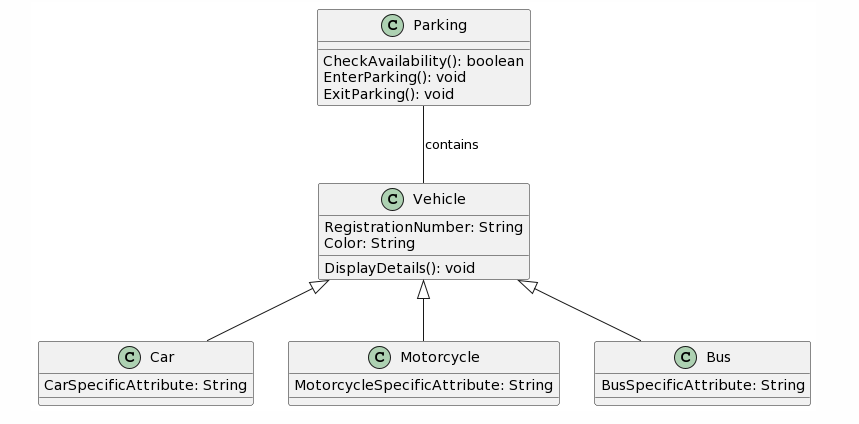
\includegraphics[width=0.75\textwidth]{photos/diagram.png}
\caption{Diagram klas systemu zarządzania parkingiem.}
\end{figure}

Struktura projektu jest zaprojektowana w taki sposób, aby maksymalizować ponowne wykorzystanie kodu i ułatwić rozszerzanie systemu o nowe funkcjonalności.
\clearpage
\section{Opis Techniczny Projektu}

Projekt został zrealizowany w języku C\#, co zapewnia szerokie możliwości w zakresie programowania obiektowego i zarządzania danymi. Do zarządzania projektem i kodem źródłowym wykorzystano środowisko Visual Studio Code z dodatkowymi wtyczkami, takimi jak PlantUML dla generowania diagramów klas UML, oraz Git jako system kontroli wersji.

System jest zaprojektowany z myślą o niskich wymaganiach sprzętowych, co czyni go dostępnym na większości współczesnych komputerów i serwerów. Minimalne wymagania to:
\begin{itemize}
    \item Procesor: 1 GHz lub szybszy.
    \item Pamięć RAM: 512 MB dla klienta, 2 GB dla serwera.
    \item Przestrzeń na dysku: 100 MB.
    \item System operacyjny: Windows 7 lub nowszy, Linux, MacOS.
\end{itemize}

Projekt wykorzystuje mechanizm zarządzania danymi oparty na bazie danych w pliku tekstowym (txt), co pozwala na prostą i efektywną manipulację danymi bez potrzeby korzystania z zewnętrznych systemów DBMS. Taki wybór umożliwia łatwą portowalność i minimalizuje wymagania sprzętowe oraz konfiguracyjne. Struktura plików tekstowych jest zaprojektowana w taki sposób, aby umożliwić szybkie odczytywanie i zapisywanie stanu miejsc parkingowych oraz informacji o pojazdach, co zapewnia wysoką wydajność działania systemu.

\section{Repozytorium i System Kontroli Wersji}

Projekt wykorzystuje system kontroli wersji Git, co umożliwia skuteczne zarządzanie historią zmian kodu źródłowego. Repozytorium kodu znajduje się na platformie GitHub pod adresem:\\ \url{https://github.com/filwalu/ProjektOOP} i będzie dostępne publicznie do dnia 30.09.2024. Bezpieczne\\ połączenie z repozytorium zabezpieczono za pomocą pary kluczy SSH. Poniżej przedstawiono opis\\ użytych poleceń Git:

\begin{enumerate}
    \item \texttt{git init} - inicjalizacja nowego repozytorium Git.
    \item \texttt{git clone [URL]} - klonowanie repozytorium przy użyciu SSH.
    \item \texttt{git add -Av} - dodawanie zmian do kolejki commitów.
    \item \texttt{git status} - sprawdzanie statusu zmian.
    \item \texttt{git commit -m "[wiadomość]"} - commitowanie zmian z opisem.
    \item \texttt{git push} - wysyłanie zmian do zdalnego repozytorium przez SSH.
\end{enumerate}
\newpage
\chapter{Harmonogram Realizacji Projektu}

Harmonogram realizacji projektu został zaplanowany z wykorzystaniem diagramu Gantta, który ilustruje kluczowe etapy rozwoju projektu, ich zależności czasowe oraz alokację zasobów. Poniżej przedstawiono diagram Gantta dla projektu System Zarządzania Parkingiem.

\begin{figure}[H]
\centering
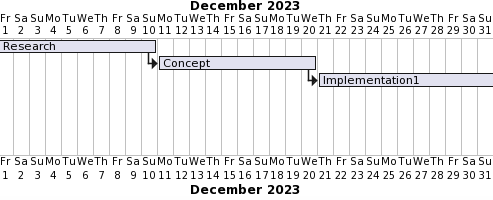
\includegraphics[width=\textwidth]{photos/gant1.png}
\caption{Diagram Gantta projektu System Zarządzania Parkingiem.}
\end{figure}
\begin{figure}[H]
\centering
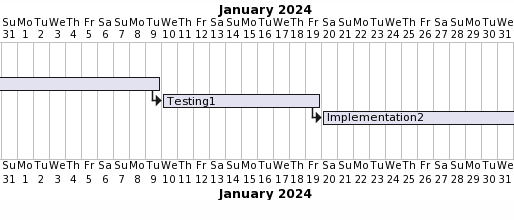
\includegraphics[width=\textwidth]{photos/gant2.png}
\caption{Diagram Gantta projektu System Zarządzania Parkingiem.}
\end{figure}
\begin{figure}[H]
\centering
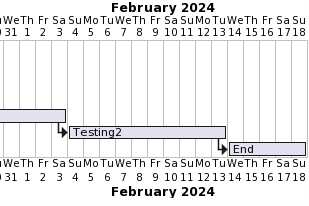
\includegraphics[width=0.80\textwidth]{photos/gant3.png}
\caption{Diagram Gantta projektu System Zarządzania Parkingiem.}
\end{figure}

\newpage
\chapter{Prezentacja warstwy użytkowej projektu}

\section{Warstwa Użytkowa Projektu}

Projekt Systemu Zarządzania Parkingiem oferuje intuicyjny i prosty w obsłudze interfejs użytkownika, który umożliwia szybkie zarządzanie miejscami parkingowymi oraz monitorowanie dostępności przestrzeni parkingowej. Interfejs użytkownika został zaprojektowany z myślą o zapewnieniu maksymalnej użyteczności i dostępności funkcji.

Aplikacja umożliwia użytkownikom wykonanie następujących akcji:
\begin{itemize}
    \item Sprawdzenie dostępności miejsc parkingowych.
    \item Rejestracja wjazdu i wyjazdu pojazdów.
    \item Zarządzanie danymi pojazdów.
\end{itemize}

Interfejs skupia się na minimalizmie i łatwości nawigacji, co pozwala na szybkie odnalezienie potrzebnych informacji i funkcji.

W tej sekcji zostaną umieszczone zrzuty ekranu przedstawiające kluczowe funkcjonalności aplikacji oraz jej interfejs użytkownika.

\begin{figure}[H]
\centering
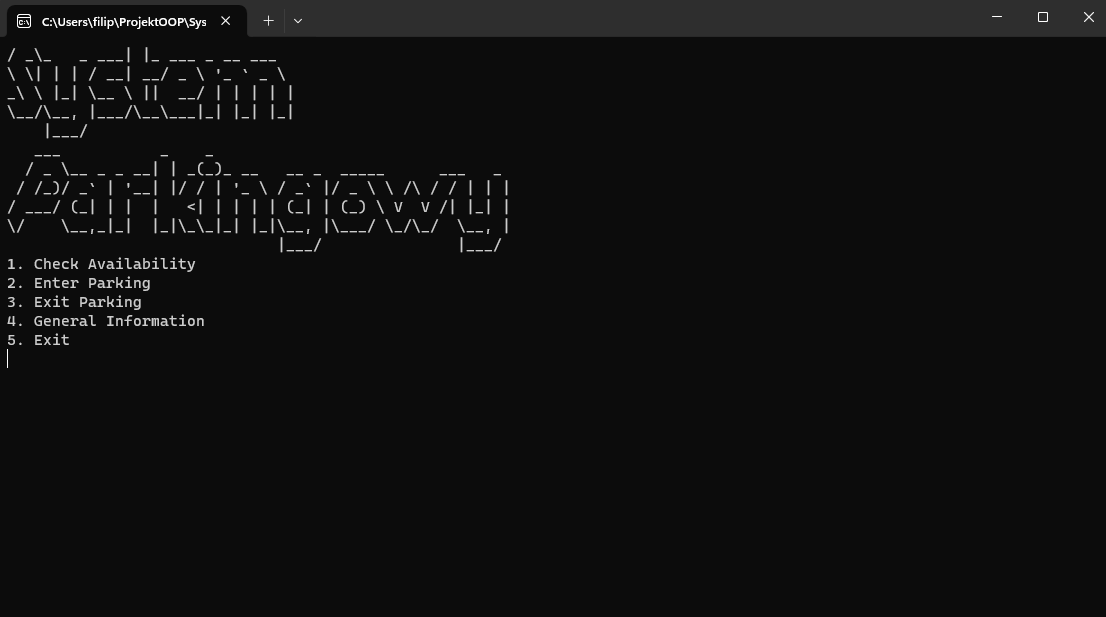
\includegraphics[width=\textwidth]{photos/mainmenu.png}
\caption{Widok głównego menu aplikacji.}
\end{figure}

W tej sekcji omówione zostaną kluczowe funkcjonalności aplikacji Systemu Zarządzania Parkingiem oraz instrukcje dotyczące ich używania.

\begin{itemize}
    \item \textbf{Sprawdzanie dostępności miejsc parkingowych} (\textit{Check Availability}):
    Użytkownik może sprawdzić dostępność miejsc parkingowych dla samochodów, wybierając opcję "1". 

    \begin{figure}[H]
    \centering
    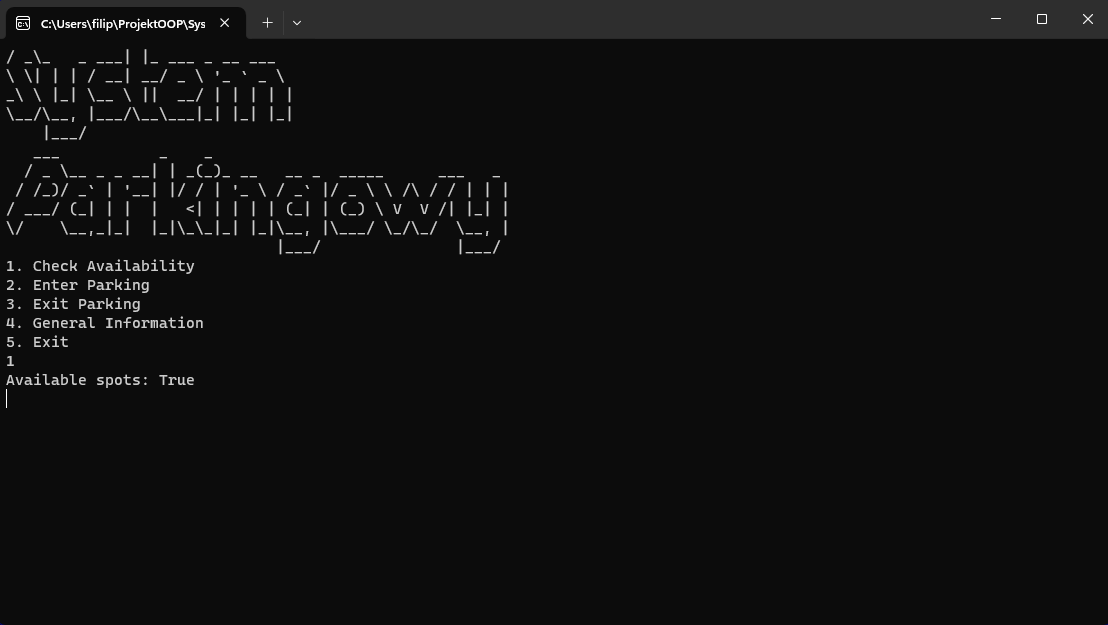
\includegraphics[width=\textwidth]{photos/avail.png}
    \caption{Opcja 1 - Check Availability.}
    \end{figure}

    \item \textbf{Wprowadzanie pojazdów na parking}:
    Użytkownik może wprowadzić pojazd na parking, wybierając opcję "2". Następnie należy podać numer rejestracyjny pojazdu, jego kolor oraz wybrać typ pojazdu (1 - Samochód, 2 - Motocykl, 3 - Autobus). Na podstawie podanych informacji, system tworzy odpowiedni obiekt pojazdu i rejestruje go w systemie parkingowym. 
        \begin{figure}[H]
        \centering
        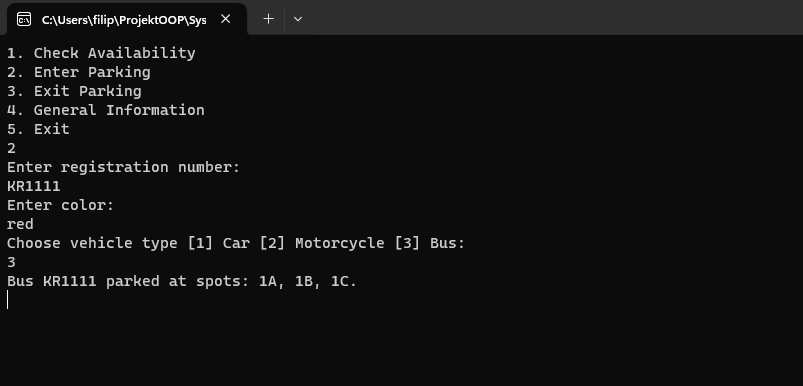
\includegraphics[width=\textwidth]{photos/enter.png}
        \caption{Opcja 2 - Enter Parking.}
        \end{figure}
    \clearpage
    \item \textbf{Wyjazd pojazdów z parkingu}:
    Użytkownik może wyjechać pojazdem z parkingu, wybierając opcję "3". Następnie należy podać numer rejestracyjny pojazdu. Na podstawie podanej informacji, system usuwa pojazd z rejestru parkingowego. 
    \begin{figure}[H]
        \centering
        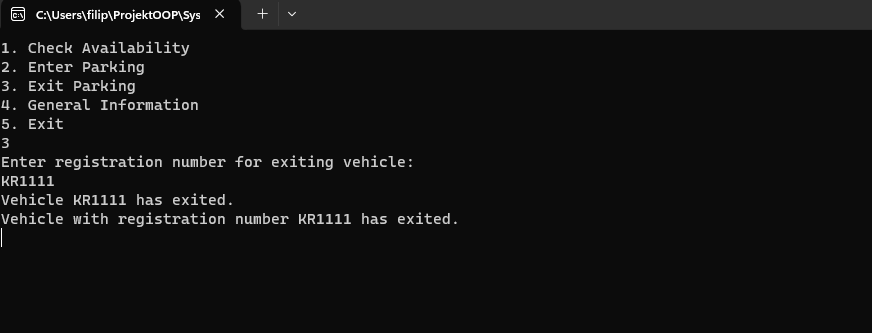
\includegraphics[width=\textwidth]{photos/exit.png}
        \caption{Opcja 3 - Exit Parking.}
        \end{figure}
    \item \textbf{Dodatkowe informacje}:
    Użytkownik wybierając opcję "4"\ wyświetla dodatkowe informacje o systemie.
        \begin{figure}[H]
        \centering
        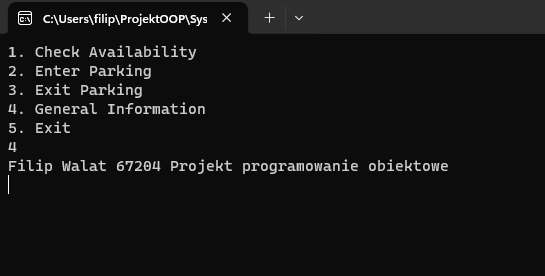
\includegraphics[width=\textwidth]{photos/info.png}
        \caption{Opcja 4 - General Information.}
        \end{figure} 
\item \textbf{Koniec}:
    Użytkownik wybierając opcję "5"\ zamyka aplikacje.
\end{itemize}
\clearpage
\section{Opis interakcji z użytkownikiem}
Sekcja ta zawiera informacje na temat interakcji z użytkownikiem, w tym otrzymywanych komunikatów, alertów oraz sposobu obsługi błędów. Poniżej przedstawiono wybrane komunikaty wyświetlane przez aplikację:

\begin{itemize}
    \item \texttt{"Available spots: [True lub False]"} - informacja mówiąca czy znajdują się obecnie wolne miejsca parkingowe.
    \item \texttt{"Enter registration number:"} - monit o wprowadzenie numeru rejestracyjnego pojazdu.
    \item \texttt{"Enter color:"} - prośba o podanie koloru pojazdu.
    \item \texttt{"Choose vehicle type [1] Car [2] Motorcycle [3] Bus:"} - wybór typu pojazdu do wprowadzenia na parking.
    \item \texttt{"Invalid vehicle type selected."} - komunikat o błędnym wyborze typu pojazdu.
    \item \texttt{"Vehicle entered the parking."} - informacja o pomyślnym wprowadzeniu pojazdu na parking.
\end{itemize}

\newpage
\chapter{Podsumowanie}
W ramach projektu Systemu Zarządzania Parkingiem wykonano szereg prac, w tym:
\begin{itemize}
    \item Projektowanie i implementacja klas reprezentujących pojazdy (samochody, motocykle, autobusy) oraz parking.
    \item Rozwój funkcjonalności zarządzania miejscami parkingowymi, w tym sprawdzanie dostępności, rejestracja wjazdu i wyjazdu pojazdów.
    \item Przygotowanie interfejsu użytkownika w konsoli do interakcji z systemem.
    \item Wykorzystanie plików tekstowych do prostego zarządzania danymi.
\end{itemize}

W dalszej kolejności planowane są następujące prace rozwojowe:
\begin{itemize}
    \item Zastosowanie klasycznej bazy danych SQL, np. PostgreSQL, dla lepszego zarządzania danymi i wydajności.
    \item Konteneryzacja aplikacji z wykorzystaniem Docker, co ułatwi wdrożenie i skalowalność.
    \item Implementacja systemu płatności.
    \item Usprawnienia interfejsu użytkownika, w tym rozwój graficznego interfejsu użytkownika (GUI) dla lepszej dostępności i ergonomii.
    \item Rozbudowa obsługi wyjątków dla zwiększenia stabilności i niezawodności aplikacji.
    \item Implementacja możliwości generowania raportów w formacie CSV z danych przechowywanych w systemie dla ułatwienia analizy i zarządzania.
\end{itemize}

\newpage

% *************** Bibliografia ***************
\begin{thebibliography}{9}

\bibitem{gitpro}
Scott Chacon, Ben Straub. \textit{Pro Git}. Apress, 2014. Dostępne online: \url{https://git-scm.com/book/en/v2}

\bibitem{dotnetdocs}
Dokumentacja Microsoft .NET. Microsoft, dostęp online: \url{https://docs.microsoft.com/en-us/dotnet/}

\bibitem{csharpstudy}
Albahari, Joseph, Albahari, Ben. \textit{C\# 7.0 in a Nutshell: The Definitive Reference}. O'Reilly Media, 2017.

\end{thebibliography}
\newpage

% *************** Zakończenie ***************
\addcontentsline{toc}{chapter}{Spis rysunków}
\listoffigures
\newpage


\end{document}
% *************** Koniec pliku szablon.tex ***************
